\documentclass{article}
\usepackage[utf8]{inputenc}
\usepackage[portuguese]{babel}
\usepackage[margin=2.5cm]{geometry}
\setlength{\parskip}{1mm}
\setlength{\parindent}{10mm}
\linespread{1.2}
\usepackage[usenames,dvipsnames,svgnames,table]{xcolor}
\usepackage{fancyhdr}
\usepackage[symbol]{footmisc}
\usepackage{amsfonts,amsmath,amssymb,amsthm}
\newtheorem{thm}{Teorema}[]
\usepackage{array,caption,graphicx}
\usepackage[shortlabels]{enumitem}
\usepackage{verbatim}
\usepackage{listings}
\usepackage{float}
\usepackage{graphicx}
\definecolor{codegreen}{rgb}{0,0.6,0}
\definecolor{codegray}{rgb}{0.5,0.5,0.5}
\definecolor{codepurple}{rgb}{0.58,0,0.82}
\definecolor{backcolour}{rgb}{0.95,0.95,0.92}
\lstdefinestyle{mystyle}{
  backgroundcolor=\color{backcolour},   commentstyle=\color{codegreen},
  keywordstyle=\color{magenta},
  numberstyle=\tiny\color{codegray},
  stringstyle=\color{codepurple},
  basicstyle=\footnotesize,
  breakatwhitespace=false,
  breaklines=true,
  captionpos=b,
  keepspaces=true,
  numbers=left,
  numbersep=5pt,
  showspaces=false,
  showstringspaces=false,
  showtabs=false,
  tabsize=2
}
\renewcommand{\thefootnote}{\arabic{footnote}}
\lstset{style=mystyle}


\title{\textbf{Análise Numérica\\Relatório 3 - Aproximação de funções}}
\author{\textbf{Grupo 29}\\[4mm]José Dias\\Luís Pinto\\Samuel Neves\\Bárbara Gonçalves\\}
\date{29 de Abril de 2019}
\begin{document}
\maketitle
\clearpage
\pagestyle{fancy}
\fancyhf{}
\setlength{\headheight}{30pt}
\rhead{Relatório nº3}
\lhead{\textbf{Grupo 29}}
\setlength{\footskip}{15pt}
\rfoot{\thepage}
\section{Introdução}
\hspace{6mm}Com este trabalho, pretendemos aproximar uma função por interpolação polinomial e spline cúbico natural de modo a encontrar uma boa aproximação duma função dada. Iremos, também, encontrar um possível valor para a imagem de uma dada abcissa sendo conhecidos pontos que pertencem a dados fornecidos. Todos os polinómios obtidos estão em forma encaixada e utilizámos a libraria \textit{sympy}, do python, para encontrar essa forma.
\begin{enumerate}
  \item{A linguagem utilizada foi Python e, portanto, os cálculos foram feitos em dupla precisão.}
  \item{Para a auxiliar a resposta ao problema em questão serão usados alguns dos seguintes métodos:}
  \begin{enumerate}
    \item[\textbullet]{Resolução Teórica;}
    \item[\textbullet]{Código do programa;}
    \item[\textbullet]{Gráficos\footnote{Dentro das mesmas alíneas representámos os gráficos com as mesmas escalas para observar melhor as diferenças entre cada gráfico.};}
    \item[\textbullet]{Tabelas;}
    \item[\textbullet]{Comentários.}

  \end{enumerate}
\end{enumerate}
\section*{Exercício 1.}
\textbf{Alínea a):}
\begin{lstlisting}[language=Python]
#Trabalho 3
import numpy as np
import sympy as sp
import math
x = sp.symbols('x')
#METODO LAGRANGE (alinea (a))
def lagrange(X,Y):
    L=[]
    pol = []
    for i in range(len(X)):
        p = ''
        d = ''
        for j in range(len(X)):
            if i != j:
                p += '(x-'+str(X[j])+')*'
                d += '('+str(X[i])+'-'+str(X[j])+')*'
        p = p[:-1]
        d = d[:-1]
        L.append(p+'/('+d+')')
    for i in range(len(L)):
        pol += L[i]+'*'+str(Y[i])+'+'
    return sp.horner(''.join(pol[:-1]))
\end{lstlisting}
\textbf{Alínea b):}
\begin{lstlisting}[language=Python]
#SPLINE CUBICO NATURAL (alinea (b))
import numpy as np
import sympy as sp
def h(L,i):
    return L[i]-L[i-1]
def spline(XL,YL):
    MM = [[1]+(len(XL)-1)*[0]]
    Lista = [0]
    hi = h(XL,1)
    for i in range(1,len(XL)-1):
        MM.append([])
        Lista.append([])
        hi1 = h(XL,i+1)
        MM[-1] = ((i-1)*[0] + [hi/6,(hi+hi1)/3,hi1/6] + (len(XL)-i-2)*[0])
        Lista[-1] = ((YL[i+1]-YL[i])/hi1)-((YL[i]-YL[i-1])/hi)
        hi = hi1
    MM.append([])
    MM[-1] = (len(XL)-1)*[0]+[1]
    Lista += [0]
    M1 = np.matrix(MM)
    M2 = np.matrix(Lista)
    M = (np.linalg.solve(M1,np.transpose(M2)))
    S = []
    for i in range(1,len(XL)):
        hi = XL[i]-XL[i-1]
        c = YL[i-1]-(M[i-1]*(hi**2))/6
        d = YL[i]-(M[i]*(hi**2)/6)
        S.append([])
        S[-1] = (M[i-1]*(XL[i]-x)**3)/(6*hi) + (M[i]*(x-XL[i-1])**3)/(6*hi) + c*(XL[i]-x)/hi + (d*(x-XL[i-1]))/hi
    for i in range(len(S)):
        print('S%d =' % (i+1),sp.horner(S[i]))
    return S

\end{lstlisting}
\section*{Exercício 2.}
\subsection*{alínea a)}
\begin{center}
\begin{tabular}{c|c c c c c c}


    $ x_{i} $ & $0$ & $1$ & $2$ & $2.5$ & $3$ & $4$ \\
    \hline
    $f_{i}$ & $1.4$ & $0.6$ & $1.0$ & $0.6$ & $0.6$ &$1.0$\\

\end{tabular}
\end{center}
\textbf{Output do programa:}
\begin{lstlisting}[language=Python]
>>> XL = [0,1,2,2.5,3,4]
>>> YL = [1.4,0.6,1.0,0.6,0.6,1.0]
>>> lagrange(XL,YL)
x*(x*(x*(x*(-0.202222222222222*x + 2.17222222222222) - 8.31111111111111) + 13.3611111111111) - 7.82) + 1.4
>>> S = spline(XL,YL)
S1 = x*(0.461410788381743*x**2 - 1.26141078838174) + 1.4
S2 = x*(x*(-1.10705394190871*x + 4.70539419087137) - 5.96680497925311) + 2.96846473029046
S3 = x*(x*(2.39336099585062*x - 16.2970954356846) + 36.0381742738589) - 25.0348547717842
S4 = x*(x*(-1.01908713692946*x + 9.29626556016598) - 27.9452282157676) + 28.2846473029046
S5 = x*(x*(-0.04149377593361*x + 0.49792531120332) - 1.55020746887967) + 1.8896265560166
\end{lstlisting}
\textbf{Nota:} Os polinómios obtidos não estão com coeficientes exatos pelo facto do computador arredondar os cálculos intermédios. Assim, ao se calcular $p_5(x_i)$, não se obtém exatamente $f_i$ mas sim uma aproximação.
\newpage
\begin{flushleft}
  \textbf{Resposta:} Usando o método de Lagrange e o método de spline cúbico natural, obtivemos o seguinte polinómio e spline:
\end{flushleft}
\[p_{5}(x) = x(x(x(x(-0.202222222222222x+2.17222222222222)-8.31111111111111)+13.3611111111111)-7.82)+1.4\]
\[S(x) = \begin{cases}
x(0.461410788381743x^2 - 1.26141078838174) + 1.4 , x\in[0,1]\\
x(x(-1.10705394190871x + 4.70539419087137) - 5.96680497925311) + 2.96846473029046, & 1\leq x\leq 2 \\
x(x(2.39336099585062x - 16.2970954356846) + 36.0381742738589) - 25.0348547717842, & 2\leq x\leq 2.5\\
x(x(-1.01908713692946x + 9.29626556016598) - 27.9452282157676) + 28.2846473029046, & 2.5\leq x\leq 3\\
x(x(-0.04149377593361x + 0.49792531120332) - 1.55020746887967) + 1.8896265560166, & 3\leq x\leq 4\\
\end{cases}\]
Onde $p_5(x)$ é o polinómio obtido pelo método de Lagrange e $S(x)$ o spline cúbico natural associado aos pontos dados.\\[3mm]
\textbf{Gráficos:}
\begin{figure}[H]
\begin{center}
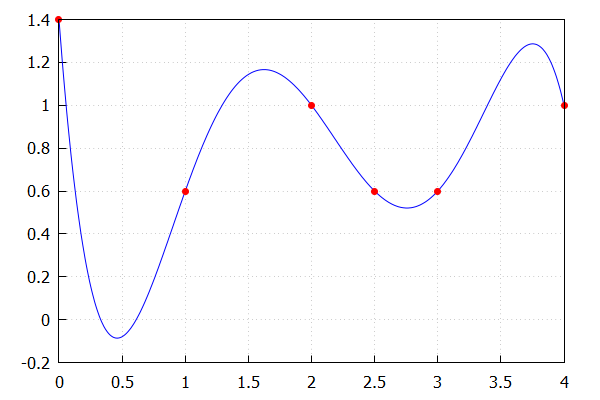
\includegraphics[scale=0.3]{./image1.png}
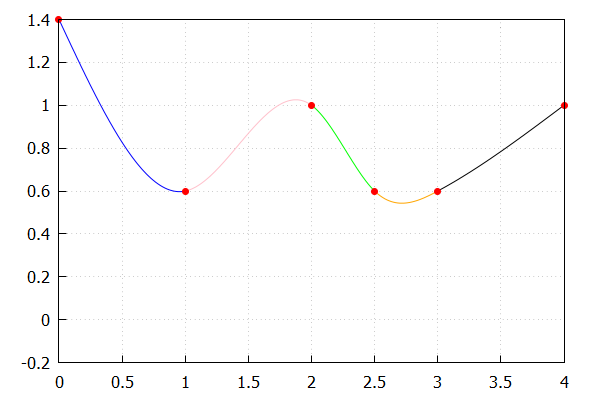
\includegraphics[scale=0.3]{./image2.png}
\caption*{Gráfico $p_5(x)$.\hspace{40mm} Gráfico $S(x)$.}
\end{center}
\end{figure}
\begin{flushleft}
\textbf{Análise gráfica:}\\
Analisando ambos os gráficos, $p_5(x)$ e $S(x)$, podemos observar que $p_5[0,1]\subset [-0.2,1.4]$ e $S[0,1]\subset [0.5,1.4]$. Assim, reparámos que o polinómio interpolador se "afasta" muito mais do ponto $(1,0.6)$ do que o spline cúbico natural, o que pode, por sua vez, dar aproximações não muito boas de valores para $x\in[0,1]$. O mesmo acontece nos restantos pontos e, portanto, é provável que $S(x)$ seja uma melhor aproximação da função com os valores tabelados do que $p_5(x)$.

\end{flushleft}
\subsection*{alínea b)}
\subsubsection*{i.}
\textbf{Código utilizado:}
\begin{lstlisting}[language=Python]
>>> from math import *
>>> def f(x):
    return 4*x**2+sin(9*x)
>>> lista = [-1,-0.75,-0.5,-0.25,0,0.25,0.5,0.75,1]
>>> for i in lista:
    print(i,f(i))
-1 3.5878815147582435
-0.75 1.7999559262193823
-0.5 1.977530117665097
-0.25 -0.5280731968879212
0 0.0
0.25 1.028073196887921
0.5 0.02246988233490299
0.75 2.7000440737806177
1 4.4121184852417565
\end{lstlisting}
\textbf{Resposta:} Obtém-se os pontos$(x_{i},f(x_{i})), \forall i \in \{0,1,...,8\},$ pela ordem acima indicada no output do programa escrito em \textbf{i}.

\subsubsection*{ii.}
\textbf{Output do programa para o polinómio interpolador:}
\begin{lstlisting}[language=Python]
>>> def f(x):
    return 4*x**2 + np.sin(9*x)
>>> lagrange([-1,-0.75,-0.5,-0.25,0,0.25,0.5,0.75,1],[f(-1),f(-0.75),f(-0.5),f(-0.25),f(0),f(0.25),f(0.5),f(0.75),f(1)])
x*(x*(x*(x*(x*(x*(x*(2.1316282072803006e-14*x - 87.33774786619881) - 3.7636560534792807e-14) + 146.82505656270518) + 1.6958656701149266e-14) - 65.7442883348996) + 3.9999999999999975) + 6.6690981236349886)
\end{lstlisting}
\textbf{Output do programa para o spline cúbico:}
\begin{lstlisting}[language=Python]
>>> def f(x):
    return 4*x**2 + np.sin(9*x)
>>> spline([-1,-0.75,-0.5,-0.25,0,0.25,0.5,0.75,1],[f(-1),f(-0.75),f(-0.5),f(-0.25),f(0),f(0.25),f(0.5),f(0.75),f(1)])
S1 = x*(x*(49.3330388667433*x + 147.99911660023) + 137.764099316903) + 42.6859030981746
S2 = x*(x*(-120.873208414704*x - 234.964939783026) - 149.458942970539) - 29.1198574736858
S3 = x*(x*(136.644448489139*x + 151.311545572739) + 43.6792997073436) + 3.0698496392946
S4 = x*(x*(-59.8259284257152*x + 3.95876288659794) + 6.84110403580837)
S5 = x*(x*(-59.4960315184987*x + 3.95876288659794) + 6.84110403580837)
S6 = x*(x*(135.65475776749*x - 142.404329077894) + 43.4318770269312) - 3.04923108259357
S7 = x*(x*(-117.244342435322*x + 236.944321226325) - 146.242448125178) + 28.5631564427579
S8 = x*(x*(35.807265670867*x - 107.421797012601) + 112.032140554016) - 36.0054907270406
\end{lstlisting}
\textbf{Gráficos:}
\begin{figure}[H]
  \begin{center}
  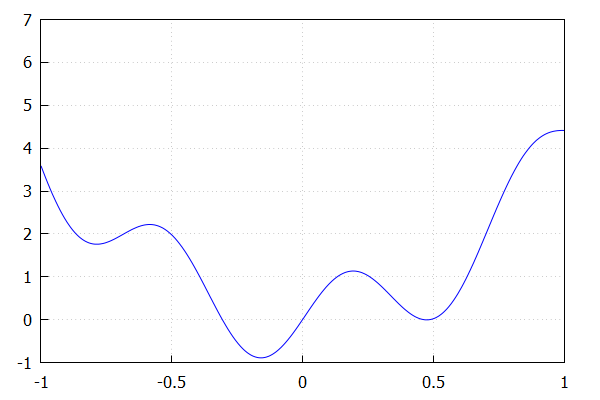
\includegraphics[scale = 0.35]{./image3.png}
  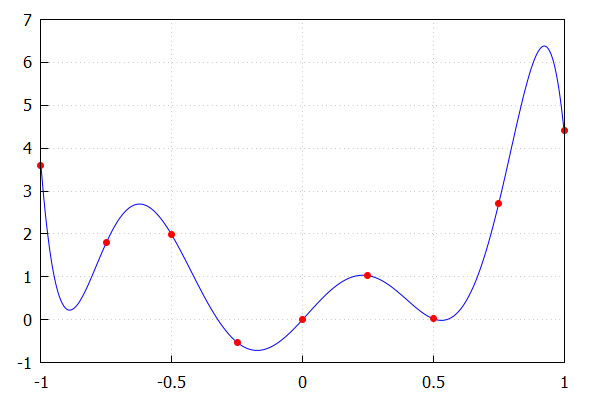
\includegraphics[scale = 0.35]{./image4.png}
  \caption*{Gráfico $f(x)$.\hspace{45mm} Gráfico polinómio interpolador $p_8(x)$.}
  \end{center}
\end{figure}
\begin{figure}[H]
  \begin{center}
  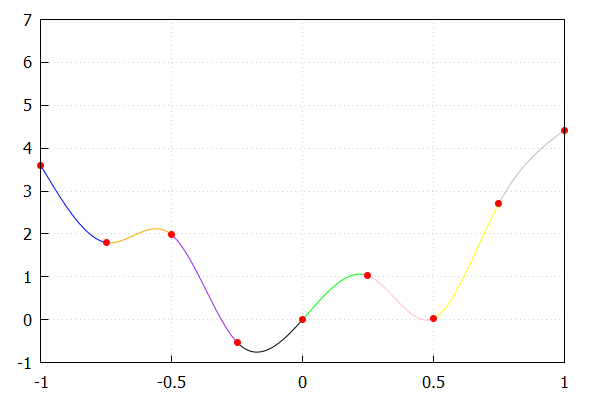
\includegraphics[scale = 0.35]{./image5.png}
  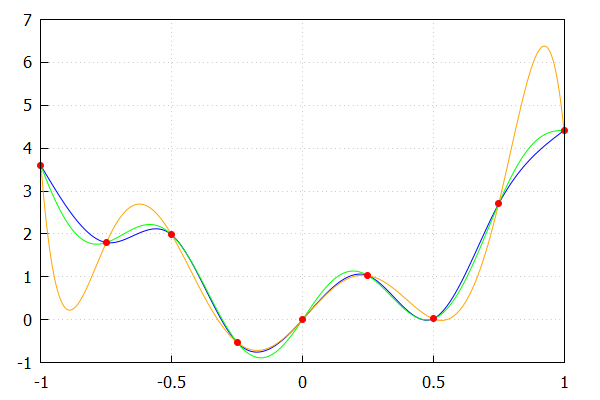
\includegraphics[scale = 0.35]{./image6.png}
  \caption*{Gráfico spline cúbico natural $S(x)$. \hspace{25mm} Gráfico com \textcolor{green}{$f(x)$}, \textcolor{orange}{$p_8(x)$} e \textcolor{blue}{$S(x)$}.}
\end{center}
\end{figure}
\begin{flushleft}
  \textbf{Análise gráfica:} \\
  Analisando os gráficos $f(x), p_{8}(x)$ e $S(x)$, verificamos que o spline cúbico natural constitui uma melhor aproximação da função $f(x)$, que é dada o que nos permite retirar uma observação direta.
\end{flushleft}
\subsubsection*{iii.}
\textbf{Resolução teórica:} Pelo teorema do erro na interpolação polinomial  tem-se que:
\[
\forall x  \in  [-1,1] \exists c_{x}  \in  ]-1,1[ :   f(x)-p_{8}(x)= \frac{1}{9!}f^{(9)}(c_{x})\pi_{9}(x)
\]
onde $\pi_{9}(x)= \prod_{i = 0}^{8}(x-x_{i})$.\\
Assim, para obter o majorante do erro cometido,$|E(x)|$, ao estimar $f(x), \forall x \in \{0.3,0.83\}$ ,basta calcular :
\[
|E(x)|=|f(x)-p_{8}(x)| \leq \frac{max_{x \in [-1,1]} |f^{(9)}(x)|}{9!}|\pi_{9}(x)|
\]
Para calcular o erro cometido usando o método do spline cúbico natural ao calcular $f(x)$ basta calcular:
\[
|E(x)|= |f(x)-S(x)| \leq \frac{5}{384}M\times h^{4}
\]
onde $M = max_{x\in[-1,1]}|f^{(4)}(x)|, h= max(h_{i}) = max(x_{i}-x_{i-1}), \forall i \in \{1,2,\dots,8\}$
\\[5mm]
\textbf{Cálculo do erro polinómio interpolador:}\\[2mm]
$f^{(9)}(x) = 9^{9}cos(9x) ; max_{x \in [-1,1]} |f^{(9)}(x)| = 9^{9}$
\begin{itemize}
  \item{$|E(0.3)| \leq \frac{9^{9}}{9!}|\pi_{9}(0.3)| \leq 6.1\times10^{-1}$}
  \item{$|E(0.83)| \leq \frac{9^{9}}{9!}|\pi_{9}(0.83)| \leq 9.6$}
\end{itemize}
\textbf{Cálculo do erro spline cúbico natural:}\\
$M = max_{x\in[-1,1]}|f^{(4)}(x)| = 9^{4}  ; h = 0.25$
\begin{itemize}
  \item{$|E(0.3)| \leq \frac{5}{384}\times 9^{4} \times0.25^{4} \leq 3.4\times10^{-1}$}
  \item{$|E(0.83)| \leq  3.4\times10^{-1} $}
\end{itemize}
%\newpage
\subsubsection*{iv.}
\textbf{Comentários:}
\begin{itemize}
\item{Melhor aproximação:\\
Analisando os gráficos em \textbf{ii.}  verificamos que o spline cúbico natural obtido constitui uma melhor aproximação da função $f(x)$ do que o polinómio interpolador e esta observação pode ser confirmada pelo cálculo da majoração do erro em \textbf{iii.}, pois $3.4\times10^{-1}<6.1\times10^{-1}<9.6$.}
\item{Cálculo do erro:\\
Note-se que $\frac{1}{9!}max_{x \in [-1,1]} |f^{(9)}(x)| = 9^{9}>1000$ é um valor muito elevado, para o erro ser baixo, $\pi_9(x)$ têm de ser bastante baixo, o que só acontece quando $x$ está próximo de algum $x_i$. Devido a este facto, como $min_{i\in\{0,...,8\}}|0.83-x_i|=0.08>0.05=min_{i\in\{0,...,8\}}|0.30-x_i|$, é esperado que $|E(0.83)|>|E(0.30)|$. Ao utilizar outro conjunto de intervalos, é provável que a aproximação por polinómio interpolador fosse mais precisa, mas isso não acontece com os nossos intervalos.}
\end{itemize}
\end{document}
